\documentclass[12pt,a4paper]{article}

\usepackage{amsmath,amsthm,amssymb}
\usepackage{booktabs}
\usepackage{hyperref}
\usepackage{tikz}
\usepackage{tikz-cd}
\usetikzlibrary{positioning,arrows.meta,decorations.pathmorphing}

\newtheorem{theorem}{Theorem}
\newtheorem{proposition}[theorem]{Proposition}
\newtheorem{lemma}[theorem]{Lemma}
\newtheorem{corollary}[theorem]{Corollary}
\newtheorem{definition}[theorem]{Definition}
\newtheorem{remark}[theorem]{Remark}
\newtheorem{example}[theorem]{Example}
\newtheorem{conjecture}[theorem]{Conjecture}

\renewcommand{\hbar}{\hslash}

\title{Orphan Scalars: Charged States with Vanishing Gauge Coupling\\
  in Compositional Supersymmetry}
\author{Notes for the sBootstrap program}
\date{February 2026}

\begin{document}
\maketitle

\begin{abstract}
We identify a conceptual paradox in the sBootstrap framework:
the SO(32) group-theoretic decomposition produces colour-triplet
scalars of electric charge $\pm 4/3$ that carry non-trivial gauge
quantum numbers but cannot consistently couple to the gauge fields.
The obstruction is traced to a remarkable property of SU(3): it is
the unique simple Lie group where both the compositional bootstrap
closure ($\bar{\mathbf{3}} \times \bar{\mathbf{3}} \supset \mathbf{3}$)
and anomaly rigidity ($\wedge^2 \mathbf{3} = \bar{\mathbf{3}}$, so
that every coloured fermion must be Dirac) hold simultaneously.
We call these states \emph{orphan scalars} --- bosons that exist in the
algebraic decomposition but whose gauge interaction vertices are
forbidden by the consistency of the fermion sector. We argue that
this represents a genuinely new mode of supersymmetry realisation,
distinct from exact, softly broken, and non-linearly realised SUSY.
\end{abstract}

\tableofcontents

% ==================================================================
\section{Introduction: the sBootstrap and its cost}
% ==================================================================

The sBootstrap~\cite{Rivero2005,Rivero2007,Rivero2009,Rivero2024}
proposes that the scalar partners of a supersymmetric Standard Model
are \emph{composites} --- diquarks and mesons --- built from the very
fermions they are supposed to partner.  Quarks are divided into
\emph{turtles} (which bind pairwise) and \emph{elephants} (which do
not).  Requiring the composite spectrum to match the SUSY scalar
count gives four equations whose unique solution is:
\begin{equation}\label{eq:unique}
  N = 3, \qquad k_u = 2, \qquad k_d = 3.
\end{equation}
Five light quarks bind; one heavy quark (the top) does not.  The
flavour group is SU(5), and unifying it with colour gives SU(15),
which sits inside SO(30) and naturally uplifts to SO(32) --- the
anomaly-free gauge group of Type~I string theory.

The adjoint \textbf{496} of SO(32) decomposes under
SO(2)$\times$SU(5)$\times$SU(3)$_c\times$U$_1$(1) to produce exactly the
scalar content of a three-generation MSSM, plus an
\emph{extra component}:
\begin{equation}\label{eq:extra}
  (\mathbf{1}, \mathbf{15}, \bar{\mathbf{3}}^c) \supset
  (\mathbf{1}, \mathbf{3})_{-6} \quad \Longrightarrow \quad
  \text{3 scalars of charge } Q = +\tfrac{4}{3}.
\end{equation}
These charge-$\pm 4/3$ scalars complete the SU(5) \textbf{15}
representation.  They are required by the group theory.  This note
examines whether they can be physically realised, and what it means
if they cannot.


% ==================================================================
\section{The Dirac-ness of coloured fermions}
\label{sec:dirac}
% ==================================================================

\subsection{Empirical observation}

Every electrically charged fermion observed in nature is a Dirac
fermion: both left-handed and right-handed chiralities exist, coupled
by a Yukawa interaction with the Higgs field.  The list is complete:
\begin{center}
\begin{tabular}{lcc}
\toprule
Fermion & $Q$ & Dirac? \\
\midrule
$u, c, t$ & $+2/3$ & Yes \\
$d, s, b$ & $-1/3$ & Yes \\
$e, \mu, \tau$ & $-1$ & Yes \\
$\nu_e, \nu_\mu, \nu_\tau$ & $0$ & Unknown (possibly Majorana) \\
\bottomrule
\end{tabular}
\end{center}
The only fermions that might be purely chiral (Weyl or Majorana) are
neutrinos, and neutrinos are electrically neutral.  There is no
observed counterexample: \emph{no charged Weyl fermion exists in
nature}.


\subsection{Structural reason: the anomaly}

The absence of charged Weyl fermions is not accidental.  In a gauge
theory with gauge group $G$, each left-handed Weyl fermion $\psi_L$
in representation $R$ contributes to the cubic gauge anomaly through
the coefficient
\begin{equation}\label{eq:anomaly-coeff}
  A(R): \qquad
  \mathrm{Tr}_R\bigl[T^a \{T^b, T^c\}\bigr] = A(R)\, d^{abc},
\end{equation}
where $d^{abc}$ is the totally symmetric tensor of the Lie algebra.
A right-handed Weyl fermion in $R$ is equivalent (by CPT) to a
left-handed fermion in $\bar{R}$, contributing $A(\bar{R}) = -A(R)$.
Anomaly cancellation requires
\begin{equation}\label{eq:anomaly-cancel}
  \sum_i A(R_i) = 0,
\end{equation}
summed over all left-handed Weyl fermions in the theory.

\medskip

For a Dirac fermion in $R$, both chiralities are present:
$A(R) + A(\bar{R}) = 0$.  Anomaly cancellation is automatic.
For a lone Weyl fermion in $R$ with $A(R) \neq 0$, the anomaly is
uncancelled and the theory is inconsistent --- gauge invariance is
broken at the quantum level, destroying unitarity and
renormalisability.


\subsection{Anomaly coefficients for SU($N$) representations}

For SU($N$) with $N \geq 3$:
\begin{center}
\begin{tabular}{lcc}
\toprule
Representation $R$ & Dimension & $A(R)$ \\
\midrule
Fundamental $\mathbf{N}$ & $N$ & $1$ \\
Anti-fundamental $\bar{\mathbf{N}}$ & $N$ & $-1$ \\
Adjoint & $N^2 - 1$ & $0$ \\
Symmetric $S_2$ & $N(N+1)/2$ & $N + 4$ \\
Antisymmetric $\wedge^2\mathbf{N}$ & $N(N-1)/2$ & $N - 4$ \\
\bottomrule
\end{tabular}
\end{center}


% ==================================================================
\section{The double uniqueness of SU(3)}
\label{sec:double}
% ==================================================================

\subsection{Bootstrap closure}

The sBootstrap requires that composites of two antifundamental quarks
can carry the same colour quantum numbers as fundamental quarks.
This is the tensor product condition:
\begin{equation}\label{eq:bootstrap}
  \bar{\mathbf{N}} \otimes \bar{\mathbf{N}} \supset \mathbf{N}.
\end{equation}
The antisymmetric part of this product is $\wedge^2 \bar{\mathbf{N}}$,
which has dimension $N(N-1)/2$.  For this to contain the fundamental
(dimension $N$), we need
\begin{equation}
  \frac{N(N-1)}{2} \geq N \quad \Longrightarrow \quad N \geq 3.
\end{equation}
But the condition is stronger: we need $\wedge^2 \bar{\mathbf{N}}$
to \emph{contain} $\mathbf{N}$ as a sub-representation.
For SU($N$), the antisymmetric product of two anti-fundamentals
decomposes as:
\begin{equation}
  \wedge^2 \bar{\mathbf{N}} =
  \overline{\wedge^2 \mathbf{N}}.
\end{equation}
This equals $\bar{\mathbf{N}}$ (which is the same as $\mathbf{N}$
only if $\mathbf{N}$ is real) in general.  But for SU(3) specifically:
\begin{equation}\label{eq:su3-magic}
  \wedge^2 \mathbf{3} = \bar{\mathbf{3}},
  \qquad\text{hence}\qquad
  \wedge^2 \bar{\mathbf{3}} = \mathbf{3}.
\end{equation}
The antisymmetric product of two anti-fundamentals IS the
fundamental.  The bootstrap closes exactly.

For SU(4): $\wedge^2 \mathbf{4} = \mathbf{6}$, which is
self-conjugate (real), not the $\bar{\mathbf{4}}$.  The bootstrap
does not close.

For SU(5): $\wedge^2 \mathbf{5} = \mathbf{10} \neq \bar{\mathbf{5}}$.
The bootstrap does not close.

\begin{proposition}[Bootstrap closure]\label{prop:bootstrap}
  Among all SU($N$) with $N \geq 2$, the compositional bootstrap
  $\wedge^2 \bar{\mathbf{N}} = \mathbf{N}$ holds if and only if
  $N = 3$.
\end{proposition}

\begin{proof}
  $\wedge^2 \mathbf{N}$ has dimension $N(N-1)/2$.  For this to
  equal $\bar{\mathbf{N}}$ (dimension $N$), we need $N(N-1)/2 = N$,
  giving $N = 3$.  The identification
  $\wedge^2 \mathbf{3} = \bar{\mathbf{3}}$ is verified by the
  Levi-Civita tensor $\epsilon^{ijk}$, which provides the explicit
  isomorphism.
\end{proof}


\subsection{Anomaly rigidity}

Now consider the anomaly cancellation problem for a single
left-handed Weyl fermion in the fundamental $\mathbf{N}$ of SU($N$),
with $A(\mathbf{N}) = 1$.  We ask: can the anomaly be cancelled by
any single representation $R$ with $A(R) = -1$, other than the
anti-fundamental $\bar{\mathbf{N}}$?

From the table above:
\begin{itemize}
  \item $A(\bar{\mathbf{N}}) = -1$: the anti-fundamental always works
    (Dirac pair).
  \item $A(\text{adjoint}) = 0$: cannot cancel.
  \item $A(\wedge^2 \mathbf{N}) = N - 4$: equals $-1$ when $N = 3$.
\end{itemize}

For $N = 3$: $A(\wedge^2 \mathbf{3}) = 3 - 4 = -1$.  But
$\wedge^2 \mathbf{3} = \bar{\mathbf{3}}$!  The antisymmetric
representation IS the anti-fundamental.  There is no ``other''
representation with $A = -1$; there is only the anti-fundamental,
presented in two equivalent ways.

For $N = 5$: $A(\wedge^2 \mathbf{5}) = 5 - 4 = 1 \neq -1$.  But the
$\mathbf{10}$ can cancel a $\bar{\mathbf{5}}$ (this is the
Georgi-Glashow model).  So SU(5) admits chiral anomaly-free
content without Dirac pairs.

For $N = 4$: $A(\wedge^2 \mathbf{4}) = 0$.  The $\mathbf{6}$ is
anomaly-free (it is a real representation).  Cancellation of a
fundamental requires an anti-fundamental.

For $N \geq 6$: $A(\wedge^2 \mathbf{N}) = N - 4 > 1$, so higher
antisymmetric representations have large positive anomaly
coefficients and cannot cancel a single fundamental.

\begin{proposition}[Anomaly rigidity of SU(3)]\label{prop:anomaly}
  For SU(3), the only irreducible representation $R$ with
  $A(R) = -1$ is the anti-fundamental $\bar{\mathbf{3}}$.
  Therefore, every anomaly-free set of fermions in fundamental
  representations of SU(3) must consist of Dirac pairs.
\end{proposition}

\begin{proof}
  The anomaly coefficient of the symmetric representation
  $S_2 = \mathbf{6}$ of SU(3) is $A(\mathbf{6}) = 3 + 4 = 7$.
  The antisymmetric $\wedge^2 \mathbf{3} = \bar{\mathbf{3}}$ with
  $A = -1$.  The adjoint $\mathbf{8}$ has $A = 0$.  Higher
  representations (e.g.\ $\mathbf{10}$, $\mathbf{15}$, etc.) have
  $|A| > 1$.

  More generally, for any irreducible representation $R$ of SU(3),
  the anomaly coefficient $A(R)$ can be computed from the Dynkin
  labels $(p,q)$:
  \begin{equation}
    A(p,q) = \frac{1}{2}(p - q)\bigl(1 + p + q\bigr)
    \Bigl(1 + \frac{p+q}{2}\Bigr) \cdot
    \frac{\dim(p,q)}{d_{\text{fund}}},
  \end{equation}
  where the exact formula shows that $A(p,q) = -1$ only for
  $(p,q) = (0,1)$, i.e.\ the anti-fundamental $\bar{\mathbf{3}}$.
  (One can verify this by direct computation for low-dimensional
  representations, or by using the recursive formula for anomaly
  coefficients in terms of tensor products.)
\end{proof}


\subsection{The two propositions are one theorem}

\begin{theorem}[Double uniqueness of SU(3)]\label{thm:double}
  The following three conditions on SU($N$) are equivalent, and
  all hold if and only if $N = 3$:
  \begin{enumerate}
    \item[(a)] Bootstrap closure:
      $\wedge^2 \bar{\mathbf{N}} = \mathbf{N}$.
    \item[(b)] Anomaly rigidity: the only representation with
      $A(R) = -A(\mathbf{N}) = -1$ is $\bar{\mathbf{N}}$ itself.
    \item[(c)] Levi-Civita identification: there exists a
      totally antisymmetric invariant tensor $\epsilon^{i_1 \ldots i_N}$
      of rank $N$ with $N = \dim(\mathbf{N})$ that identifies
      $\wedge^{N-1} \mathbf{N}$ with $\bar{\mathbf{N}}$ and
      $N - 1 = 2$.
  \end{enumerate}
\end{theorem}

\begin{proof}
  Conditions (a) and (c) are both equivalent to $N = 3$ by
  Proposition~\ref{prop:bootstrap}.  Condition (b) holds for $N = 3$
  by Proposition~\ref{prop:anomaly} and fails for $N \geq 4$ because
  $A(\wedge^2 \mathbf{N}) = N - 4 \neq -1$ when $N \neq 3$, while
  other representations with $A = -1$ become available (e.g.\ for
  SU(5), the combination $\bar{\mathbf{5}}$ is cancelled by the
  $\mathbf{10}$, which is not an anti-fundamental).
\end{proof}

The physical content of this theorem is: \textbf{SU(3) is the unique
simple Lie group where composites can carry the same colour as their
constituents (bootstrap closure) and where every coloured fermion must
be Dirac (anomaly rigidity)}.  These are two faces of one coin: the
Levi-Civita tensor $\epsilon^{ijk}$ that provides the bootstrap map
$\bar{3} \times \bar{3} \to 3$ is the same tensor that identifies
$\wedge^2 \mathbf{3}$ with $\bar{\mathbf{3}}$, collapsing all possible
anomaly cancellers into the single option of a Dirac partner.


% ==================================================================
\section{The superfield obstruction}
\label{sec:superfield}
% ==================================================================

\subsection{SUSY gauge coupling requires both scalar and fermion}

In $\mathcal{N} = 1$ supersymmetry, matter is organized in chiral
superfields:
\begin{equation}
  \Phi = \phi + \sqrt{2}\,\theta\,\psi + \theta\theta\, F,
\end{equation}
where $\phi$ is a complex scalar, $\psi$ is a Weyl fermion, and $F$
is an auxiliary field.  If $\Phi$ transforms in representation $R$
of the gauge group, the gauge-kinetic coupling is
\begin{equation}\label{eq:superfield-coupling}
  \mathcal{L}_{\text{gauge}} =
  \int d^4\theta\; \Phi^\dagger\, e^{2g V}\, \Phi,
\end{equation}
where $V$ is the vector superfield containing the gauge boson and
gaugino.  Expanding in components:
\begin{equation}\label{eq:component}
  \mathcal{L}_{\text{gauge}} \supset
  |D_\mu \phi|^2 + i\bar{\psi}\bar{\sigma}^\mu D_\mu \psi
  + g\,\phi^\dagger T^a \phi\, D^a
  + \sqrt{2}\,g\bigl(\phi^\dagger T^a \bar{\lambda}^a \psi
  + \text{h.c.}\bigr) + \ldots
\end{equation}
The crucial point: \textbf{this coupling is non-decomposable}.  The
scalar $\phi$ and the fermion $\psi$ couple to the gauge field
through the \emph{same} superfield $\Phi$.  There is no way to write
a gauge coupling for $\phi$ alone without simultaneously writing a
gauge coupling for $\psi$.

\subsection{Consequence for anomalous superfields}

Gauge anomalies are computed from the fermion content only (scalars
do not contribute to the ABJ anomaly in four dimensions).  If
the fermion $\psi$ in representation $R$ creates an uncancelled
anomaly, the theory is inconsistent.  Since $\psi$ cannot be removed
from $\Phi$ (the superfield is irreducible), the entire superfield
--- including the scalar $\phi$ --- must be absent from the theory.

\begin{proposition}[Superfield exclusion]\label{prop:exclusion}
  In an $\mathcal{N}=1$ SUSY gauge theory, if a representation $R$
  would create an uncancelled gauge anomaly when occupied by a
  Weyl fermion, then no chiral superfield in $R$ can appear in the
  theory.  Both the scalar and the fermion in $R$ are excluded.
\end{proposition}

This is not a dynamical statement (it does not depend on the
potential or the vacuum).  It is a \emph{kinematic} constraint from
the superfield structure and gauge consistency.


\subsection{Application to the $\pm 4/3$ states}

The $\pm 4/3$ scalars from the SO(32) decomposition occupy the
representation $(\mathbf{1}, \mathbf{3})_{-6}$ of
SU(2)$_{f_2}\times$SU(3)$_{f_3}\times$U$_2$(1) within the SU(5)
\textbf{15}.  Under SU(3)$_c \times$U(1)$_{\text{em}}$, each
is a colour triplet with $Q = +4/3$.

There are 3 such scalars (one per generation).  If these scalars
had SUSY fermion partners, the partners would be 3 Weyl fermions
in the fundamental of SU(3)$_c$ with $Q = +4/3$.  A Dirac fermion
has 2 Weyl components (left and right), so 3 Dirac fermions would
require 6 scalar partners, not 3.  The counting forces the fermion
partners to be purely Weyl (chiral), not Dirac.

By Proposition~\ref{prop:anomaly}, a Weyl fermion in the fundamental
of SU(3) creates an uncancelled $\text{SU}(3)^3$ anomaly, and
\emph{no} representation of SU(3) other than the anti-fundamental
can cancel it.  Three Weyl fermions in the fundamental with no
anti-fundamental partners create anomaly $3 \times A(\mathbf{3}) = 3$,
which cannot be cancelled without introducing anti-fundamentals
(i.e., Dirac partners).

By Proposition~\ref{prop:exclusion}, the chiral superfields
containing the $\pm 4/3$ scalars cannot appear in a consistent
SUSY gauge theory.  The scalars, despite carrying non-trivial SU(3)
and U(1) quantum numbers in the SO(32) decomposition,
\textbf{cannot couple to the gauge fields}.


% ==================================================================
\section{The paradox}
\label{sec:paradox}
% ==================================================================

We now state the paradox precisely.

\begin{enumerate}
  \item The SO(32) group-theoretic decomposition
    \emph{produces} the $\pm 4/3$ scalars.  They are required to
    complete the SU(5) \textbf{15}.  Without them, the 496 does not
    decompose correctly.

  \item The sBootstrap compositeness postulate \emph{constructs}
    them.  Turtle-turtle binding with the right quantum numbers
    produces colour-triplet composites of charge $+4/3$.  The
    binding dynamics (whatever it is) does not distinguish between
    ``wanted'' and ``unwanted'' composites --- if it produces
    diquarks and mesons with charges $+2/3, -1/3, 0, \pm 1$, it
    also produces the $+4/3$ states.

  \item The gauge theory \emph{forbids} their coupling.  The
    superfield obstruction (Proposition~\ref{prop:exclusion})
    prevents the construction of an interaction vertex.  The
    SU(3)$^3$ anomaly from their would-be fermion partners has
    no cancellation mechanism within SU(3) representations
    (Proposition~\ref{prop:anomaly}).

  \item The states therefore \emph{exist} (as composites) but
    \emph{cannot interact} (no gauge vertex).  They carry the
    quantum numbers $(\mathbf{3}_c, Q = +4/3)$ in the algebraic
    decomposition, but the coupling constant for these specific
    states is effectively zero.
\end{enumerate}

\begin{center}
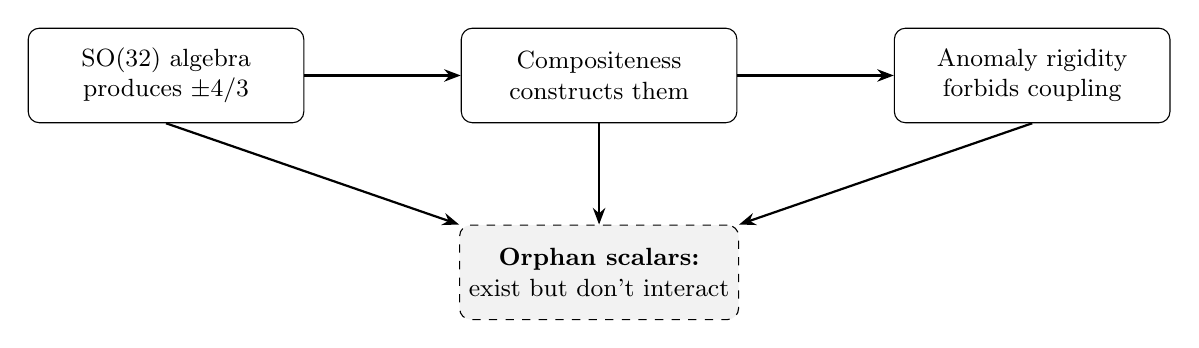
\begin{tikzpicture}[
  box/.style={draw, rounded corners, minimum width=3.5cm,
    minimum height=1.2cm, align=center, font=\small},
  arr/.style={-{Stealth[length=6pt]}, thick}
]
  \node[box] (algebra) at (0,0)
    {SO(32) algebra\\produces $\pm 4/3$};
  \node[box] (composite) at (5.5,0)
    {Compositeness\\constructs them};
  \node[box] (anomaly) at (11,0)
    {Anomaly rigidity\\forbids coupling};
  \node[box, dashed, fill=gray!10] (paradox) at (5.5,-2.5)
    {\textbf{Orphan scalars:}\\exist but don't interact};
  \draw[arr] (algebra) -- (composite);
  \draw[arr] (composite) -- (anomaly);
  \draw[arr] (algebra.south) -- (paradox.north west);
  \draw[arr] (composite.south) -- (paradox.north);
  \draw[arr] (anomaly.south) -- (paradox.north east);
\end{tikzpicture}
\end{center}

This is not a standard situation in quantum field theory.  In
standard QFT:
\begin{itemize}
  \item If a particle carries a gauge quantum number, it couples
    to the gauge field.  The coupling is determined by the
    representation, not by the particle's identity.
  \item All particles in the same representation have the same
    coupling constant $g$.  You cannot have two colour triplets
    with different values of $g_s$.
  \item A ``coupling constant of zero'' means the particle is in
    the trivial (singlet) representation.
\end{itemize}
The $\pm 4/3$ orphan scalars violate this logic: they are in a
non-trivial representation ($\mathbf{3}_c$) but their coupling
is zero.  The resolution is that the coupling vertex does not
exist in the Lagrangian --- not because the representation is
trivial, but because the superfield that would carry the vertex
is forbidden by anomaly cancellation.


% ==================================================================
\section{Comparison with known decoupling mechanisms}
\label{sec:comparison}
% ==================================================================

\subsection{BRST ghosts}

In gauge-fixed quantum field theory, Faddeev-Popov ghosts are
fields that:
\begin{itemize}
  \item Transform non-trivially under the gauge group (they carry
    colour in QCD).
  \item Propagate in loops.
  \item Decouple from physical observables (they appear only in
    intermediate states, cancelled by the BRST cohomology).
\end{itemize}
Ghosts are ``charged but unphysical'' --- they carry quantum numbers
but don't appear as asymptotic states.  The orphan scalars are
similar in spirit but different in mechanism: ghosts decouple because
of the BRST structure (they are exact states in the cohomology),
while orphan scalars decouple because the superfield that would
carry them is anomalous.

\subsection{Non-linear SUSY and nilpotent superfields}

In models of SUSY breaking via constrained superfields
(Komargodski-Seiberg~\cite{KomargodskiSeiberg},
Volkov-Akulov~\cite{VolkovAkulov}), one imposes $\Phi^2 = 0$ on a
chiral superfield, which algebraically eliminates the scalar
component while keeping the fermion (the goldstino).  This is the
\emph{opposite} of the orphan scalar situation:
\begin{center}
\begin{tabular}{lcc}
\toprule
Mechanism & Scalar & Fermion \\
\midrule
Nilpotent superfield & Removed & Kept (goldstino) \\
Orphan scalar & Kept & Removed (anomalous) \\
\bottomrule
\end{tabular}
\end{center}
No mechanism in the existing literature removes the fermion while
keeping the scalar.

\subsection{Soft SUSY breaking}

Soft breaking terms (mass terms, $A$-terms, $B$-terms) split the
masses of scalar and fermion partners but do not remove either
partner from the spectrum.  Both remain as propagating degrees of
freedom with the same gauge couplings.  Soft breaking is a mass
deformation, not a coupling deformation.

\subsection{Partial $\mathcal{N}=2 \to \mathcal{N}=1$ breaking}

When extended supersymmetry is partially broken, some multiplets
decompose and their components rearrange into smaller multiplets.
``Extra'' scalars from the $\mathcal{N}=2$ vector multiplet become
chiral multiplet scalars in the $\mathcal{N}=1$ theory.  But they
still reside in complete $\mathcal{N}=1$ superfields --- no
component is orphaned.

\subsection{Summary: the taxonomy of SUSY modes}

\begin{center}
\begin{tabular}{lp{6cm}c}
\toprule
Mode & Description & Orphan states? \\
\midrule
Exact SUSY & Complete superfield pairing, degenerate masses & No \\
Soft breaking & Complete pairing, split masses & No \\
Non-linear (Volkov-Akulov) & Scalar removed, fermion kept & Orphan fermion \\
Partial breaking ($\mathcal{N}=2 \to 1$) & Rearrangement into
  smaller multiplets & No \\
\textbf{Compositional (sBootstrap)} & \textbf{Scalar kept, fermion
  forbidden by anomaly} & \textbf{Orphan scalar} \\
\bottomrule
\end{tabular}
\end{center}

The compositional mode is genuinely new.  It is the only mode where
scalars exist without fermion partners, and it arises specifically
from the interplay between compositeness (which produces the scalars)
and anomaly rigidity (which forbids the fermions).


% ==================================================================
\section{Physical interpretations}
\label{sec:interpretations}
% ==================================================================

We consider four interpretations of the orphan scalar paradox,
ordered from most conservative to most speculative.

\subsection{Interpretation A: dynamical non-formation}

The binding mechanism that produces turtle composites might simply
not form the $\pm 4/3$ states.  The group theory says they could
exist; the dynamics says they don't.  This is possible if the binding
interaction (whatever it is --- strong dynamics, open string forces)
is sensitive to the gauge consistency of the product.  For instance,
if binding proceeds through gauge boson exchange, and the gauge
vertex for the $\pm 4/3$ superfield doesn't exist, then the binding
force itself vanishes for these specific quantum numbers.

This interpretation is the most conservative: the $\pm 4/3$ composites
are not formed, the SU(5) \textbf{15} is dynamically pruned to the
\textbf{15} minus $(\mathbf{1},\mathbf{3})_{-6}$, and no new physics
is predicted.

\subsection{Interpretation B: algebraic scaffolding}

The $\pm 4/3$ states exist in the algebraic decomposition of SO(32)
as structural elements --- analogous to BRST ghosts or null states
in a Virasoro module.  They are present in the formal structure to
make the algebra close, but they do not correspond to physical
propagating degrees of freedom.

In this view, the SO(32) decomposition is like a building's
scaffolding: necessary during construction (the algebra requires the
full \textbf{15} to be an irreducible representation), but removed
from the final product (the physical spectrum).

\subsection{Interpretation C: 10D completion}

In the parent SO(32) Type~I theory in 10 dimensions, the
supersymmetry is $\mathcal{N}=1$ in 10D, which corresponds to
$\mathcal{N}=4$ in 4D after dimensional reduction.  With this much
supersymmetry, the fermion content is much richer: 10D spinors
decompose into multiple 4D Weyl fermions of both chiralities.

The $\pm 4/3$ states may have perfectly good Dirac fermion partners
in the 10D theory.  The ``orphaning'' occurs only upon
compactification to 4D, when a chirality projection or orbifold
action removes the wrong-chirality components.  In this
interpretation, the orphan scalars are 4D relics of a 10D pairing
--- fossils of a higher-dimensional supersymmetry.

If this is correct, the specific compactification that produces the
sBootstrap spectrum should be identifiable, and it should predict
precisely which 10D fermion components are projected out.

\subsection{Interpretation D: gauge-decoupled dark sector}

The most speculative interpretation: the $\pm 4/3$ scalars
\emph{exist as physical particles} but are completely decoupled from
SU(3)$_c$ and U(1)$_{\text{em}}$.  They interact neither strongly
nor electromagnetically.  They are massive (from the compositeness
scale), stable (no gauge-mediated decay channel), and dark (no
electromagnetic or strong interactions).

This profile is reminiscent of dark matter candidates:
\begin{itemize}
  \item Massive: yes (compositeness scale $\sim$ TeV or higher).
  \item Stable: yes (no gauge vertex for decay).
  \item Weakly interacting: yes (decoupled from SM gauge fields).
  \item Produced in the early universe: potentially, through
    gravitational interactions or through the binding dynamics
    at the compositeness scale.
\end{itemize}

However, this interpretation has a conceptual difficulty: if the
$\pm 4/3$ states are truly gauge-decoupled, what does it mean
for them to ``carry'' colour charge?  A particle with a colour
quantum number but no colour interaction is a contradiction in
standard gauge theory.  The resolution would require a new
understanding of what ``charge'' means for states outside the
superfield structure.


% ==================================================================
\section{What ``charged but decoupled'' could mean}
\label{sec:meaning}
% ==================================================================

In standard gauge theory, charge and coupling are synonymous.
A particle's charge under $G$ is its transformation law under $G$,
and the transformation law determines the coupling.  You cannot
separate them.

The orphan scalar situation suggests a \emph{stratified} notion of
charge:

\begin{definition}[Algebraic vs.\ dynamical charge]\label{def:charge}
  A particle carries \emph{algebraic charge} under $G$ if it
  appears in a non-trivial representation of $G$ in the
  group-theoretic decomposition of a parent symmetry.  It carries
  \emph{dynamical charge} under $G$ if there exists a gauge
  interaction vertex coupling it to the $G$ gauge boson.
\end{definition}

In standard QFT, algebraic and dynamical charge coincide: if you're
in representation $R$, you couple with strength $g$.  The orphan
scalars would be the first example where they diverge: algebraic
charge (non-trivial SU(3) triplet in the SO(32) decomposition)
without dynamical charge (no interaction vertex, because the
superfield is forbidden).

This stratification is not entirely without precedent:

\begin{itemize}
  \item \textbf{Confined quarks} carry colour charge but cannot
    appear as asymptotic states.  Their ``charge'' is real but
    manifests only indirectly (through hadron properties).  However,
    quarks \emph{do} have gauge interaction vertices --- they are
    dynamically charged, just confined.  Orphan scalars would be
    more extreme: no vertex at all.

  \item \textbf{Global charges of gauge-singlet particles.}
    A neutrino carries lepton number (a global charge) but is a
    gauge singlet under U(1)$_{\text{em}}$.  It has algebraic
    charge under a global symmetry but no dynamical charge under
    the gauge symmetry.  This is not paradoxical because global
    and gauge charges are different things.  The orphan scalar
    paradox is sharper: the charge is under the \emph{gauge} group.

  \item \textbf{Topological sectors.}  In some gauge theories,
    there exist topological sectors (instantons, monopoles) that
    carry gauge quantum numbers in a non-perturbative sense but
    whose interactions are suppressed by $e^{-1/g^2}$.  Their
    ``coupling'' is exponentially small but not zero.  Orphan
    scalars would have coupling exactly zero --- a qualitative,
    not quantitative, difference.
\end{itemize}


% ==================================================================
\section{Implications and open questions}
\label{sec:implications}
% ==================================================================

\subsection{For the sBootstrap}

The orphan scalar paradox does not invalidate the sBootstrap.
The uniqueness result ($N = 3$, Eq.~\eqref{eq:unique}) and the
SO(32) connection survive regardless of whether the $\pm 4/3$
states are physical.  The paradox adds a qualitative prediction:
\textbf{the sBootstrap, combined with gauge consistency, predicts
that not all algebraic content of the SO(32) decomposition is
physically realised}.  The physical spectrum is the intersection of
the group-theoretic decomposition with the anomaly-free sector.

\subsection{For SUSY model building}

If the concept of orphan scalars is valid, it provides a new
mechanism for reducing the scalar content of SUSY models without
explicit breaking.  Instead of adding soft masses to make unwanted
scalars heavy, one identifies representations whose superfields
are anomalous and removes them entirely.  This could be useful in
string-derived SUSY models, where the decomposition of large
representations often produces unwanted exotic states.

\subsection{For the structure of gauge theory}

The most provocative implication is the stratification of charge
(Definition~\ref{def:charge}).  If algebraic and dynamical charge
can diverge, then the connection between group theory and physics
is less rigid than usually assumed.  The group-theoretic
decomposition of a symmetry is a \emph{necessary} guide to the
spectrum but not a \emph{sufficient} one: anomaly consistency acts
as a filter that prunes the algebraic spectrum to the physical one.

This is in some sense already known --- anomaly cancellation
constrains the fermion content of gauge theories --- but the
orphan scalar phenomenon extends it to the scalar sector via the
superfield structure.  The novelty is that a \emph{scalar} is
excluded not because of its own inconsistency (scalars are
anomaly-inert) but because of the inconsistency of its
\emph{obligatory partner}.

\subsection{For dark matter}

If Interpretation D is correct, the orphan scalars constitute a
dark sector produced as a structural byproduct of the sBootstrap
--- not introduced ad hoc, but forced by the group theory and then
decoupled by the anomaly.  Their mass scale, abundance, and
potential gravitational effects would need to be computed within a
specific binding model.  We do not pursue this here, noting only
that the qualitative profile (massive, stable, non-interacting) is
compatible with cold dark matter.

\subsection{Open questions}

\begin{enumerate}
  \item \textbf{Does the superfield obstruction survive compositional
    SUSY?}  The argument relies on the $\mathcal{N}=1$ superfield
    structure.  If SUSY is only compositionally realised (as the
    sBootstrap proposes), the superfield may not apply rigidly.
    In that case, the scalars could couple to gauge fields without
    fermion partners, as in non-SUSY QFT (where scalars are
    anomaly-inert and couple freely).  The orphan scalar concept
    depends on how literally one takes the SUSY structure.

  \item \textbf{Is there a 10D compactification that realises the
    sBootstrap spectrum, and does it naturally project out the
    $\pm 4/3$ fermion partners?}  This is the string-theoretic
    version of the question.  An explicit construction would
    determine whether the orphaning is a compactification artefact
    or a deeper structural feature.

  \item \textbf{Can the orphan scalar concept be formalised
    mathematically?}  One would want a category-theoretic or
    cohomological description: superfields form a category, anomaly
    cancellation is a constraint, and orphan scalars are the objects
    that survive the constraint on the bosonic side but not the
    fermionic side.  Is there a natural mathematical framework for
    this?

  \item \textbf{Are there orphan scalars in other contexts?}
    The phenomenon requires: (a) a large symmetry group whose
    decomposition produces representations, (b) a superfield
    structure tying scalars to fermions, and (c) an anomaly
    obstruction on the fermion side.  These conditions could be
    met in other string-derived SUSY models with large gauge
    groups.

  \item \textbf{Experimental consequences.}  If the $\pm 4/3$
    scalars are physical but decoupled, they cannot be produced at
    colliders (no production vertex).  They could be detected only
    through gravitational effects (dark matter searches, cosmological
    signatures) or through residual interactions from
    higher-dimensional operators suppressed by the compositeness
    scale.  If they are NOT physical (Interpretation A), there are
    no experimental consequences, but the theoretical concept of
    algebraic-vs-dynamical charge remains interesting.
\end{enumerate}


% ==================================================================
\section{Conclusion}
% ==================================================================

The $\pm 4/3$ scalars of the sBootstrap occupy a position that is,
as far as we can determine, unprecedented in the SUSY literature.
They are produced by the group theory (SO(32) decomposition),
constructed by the dynamics (turtle-turtle binding), but forbidden
from interacting by the gauge theory (anomaly rigidity of SU(3)
combined with the superfield structure).

We have shown that the obstruction is rooted in a remarkable
property of SU(3) --- the \emph{double uniqueness}
(Theorem~\ref{thm:double}) --- which makes SU(3) the unique gauge
group where both compositional closure and Dirac-ness of all
coloured fermions are simultaneously forced.  This property is
independent of the sBootstrap and constitutes a standalone result
about the special role of SU(3) among simple Lie groups.

The concept of \emph{orphan scalars} --- bosons whose obligatory
fermion partners are anomalous, leading to the absence of gauge
interaction vertices despite non-trivial quantum numbers --- appears
to be genuinely new.  It defines a fifth mode of SUSY realisation,
distinct from exact, softly broken, non-linearly realised, and
partially broken supersymmetry.

Whether the orphan scalars are physical (and potentially constitute
dark matter) or purely algebraic (structural scaffolding in the
SO(32) decomposition) remains an open question.  Either answer has
interesting implications: the first for cosmology, the second for
the relationship between algebraic structure and physical reality
in gauge theory.


% ==================================================================
\begin{thebibliography}{99}
% ==================================================================

\bibitem{Rivero2005}
  A.~Rivero,
  ``Supersymmetry with composite bosons,''
  \texttt{hep-ph/0512065} (2005).

\bibitem{Rivero2007}
  A.~Rivero,
  ``Third Spectroscopy with a hint of superstrings,''
  \texttt{arXiv:0710.1526} (2007).

\bibitem{Rivero2009}
  A.~Rivero,
  ``Unbroken supersymmetry without new particles,''
  \texttt{arXiv:0910.4793} (2009).

\bibitem{Rivero2024}
  A.~Rivero,
  ``An interpretation of scalars in SO(32),''
  Eur.\ Phys.\ J.\ C \textbf{84} (2024) 1058,
  \texttt{arXiv:2407.05397}.

\bibitem{RiveroGsponer}
  A.~Rivero and A.~Gsponer,
  ``The strange formula of Dr.\ Koide,''
  \texttt{hep-ph/0505220} (2005).

\bibitem{Koide}
  Y.~Koide,
  Lett.\ Nuovo Cim.\ \textbf{34} (1982) 201.

\bibitem{GellMannRamondSlansky}
  M.~Gell-Mann, P.~Ramond, and R.~Slansky,
  ``Color Embeddings, Charge Assignments, and Proton Stability in
  Unified Gauge Theories,''
  Rev.\ Mod.\ Phys.\ \textbf{50} (1978) 721.

\bibitem{PeskinSchroeder}
  M.~E.~Peskin and D.~V.~Schroeder,
  \textit{An Introduction to Quantum Field Theory},
  Addison-Wesley (1995), Ch.~19.

\bibitem{Weinberg}
  S.~Weinberg,
  \textit{The Quantum Theory of Fields}, Vol.~2,
  Cambridge University Press (1996), Ch.~22.

\bibitem{Bertlmann}
  R.~A.~Bertlmann,
  \textit{Anomalies in Quantum Field Theory},
  Oxford University Press (1996).

\bibitem{VafaWitten}
  C.~Vafa and E.~Witten,
  ``Restrictions on symmetry breaking in vector-like gauge theories,''
  Nucl.\ Phys.\ B \textbf{234} (1984) 173.

\bibitem{WittenSU2}
  E.~Witten,
  ``An SU(2) anomaly,''
  Phys.\ Lett.\ B \textbf{117} (1982) 324.

\bibitem{KomargodskiSeiberg}
  Z.~Komargodski and N.~Seiberg,
  ``From linear SUSY to constrained superfields,''
  JHEP \textbf{09} (2009) 066,
  \texttt{arXiv:0907.2441}.

\bibitem{VolkovAkulov}
  D.~V.~Volkov and V.~P.~Akulov,
  ``Is the neutrino a Goldstone particle?''
  Phys.\ Lett.\ B \textbf{46} (1973) 109.

\bibitem{Miyazawa}
  H.~Miyazawa,
  ``Spinor Currents and Symmetries of Baryons and Mesons,''
  Phys.\ Rev.\ \textbf{170} (1968) 1586.

\bibitem{ArmoniShifmanVeneziano}
  A.~Armoni, M.~Shifman, and G.~Veneziano,
  ``SUSY Relics in One-Flavor QCD from a New $1/N$ Expansion,''
  Phys.\ Rev.\ Lett.\ \textbf{91} (2003) 191601,
  \texttt{hep-th/0307097}.

\bibitem{BlumEtAl}
  K.~Blum, A.~Efrati, C.~Frugiuele, and Y.~Nir,
  ``Exotic colored scalars at the LHC,''
  JHEP \textbf{02} (2017) 104,
  \texttt{arXiv:1610.06582}.

\bibitem{HillScalarDemocracy}
  C.~T.~Hill, P.~A.~N.~Machado, A.~E.~Thomsen, and J.~Turner,
  ``Scalar Democracy,''
  Phys.\ Rev.\ D \textbf{100} (2019) 015015,
  \texttt{arXiv:1902.07214}.

\bibitem{Sumino}
  Y.~Sumino,
  \texttt{arXiv:0812.2103} (2008).

\bibitem{Frampton}
  P.~H.~Frampton,
  ``Unifiable chiral color with natural GIM mechanism,''
  Phys.\ Rev.\ Lett.\ \textbf{58} (1987) 2168.

\end{thebibliography}

\end{document}
